%% V1.0
%% by Christopher Leith, udacl@cielsystems.com
%% This is a template for Udacity projects using IEEEtran.cls

\documentclass[10pt,journal,compsoc]{IEEEtran}

\usepackage[pdftex]{graphicx}    
\usepackage{cite}
\hyphenation{op-tical net-works semi-conduc-tor}

\begin{document}

\title{MapMyWorld - Robotic Simultaneous Localization and Mapping}

\author{Christopher Leith}

\markboth{MapMyWorld, SLAM, Udacity}%
{}
\IEEEtitleabstractindextext{%

\begin{abstract}
In this project we create a simulated robot and demonstrate Simultaneous Localization and Mapping (SLAM) within the ROS framework to permit navigation within a small simulated "Gazebo" world. A differential drive robot is designed to operate within the Gazebo simulation and uses the ROS navigation stack and the RTAB-map-ros package for creating a map on the fly and localizing itself within that map.\end{abstract}

% Note that keywords are not normally used for peerreview papers.
\begin{IEEEkeywords}
Mobile Robot, SLAM, ROS.
\end{IEEEkeywords}}


\maketitle
\IEEEdisplaynontitleabstractindextext
\IEEEpeerreviewmaketitle
\label{sec:Introduction}
\section{Introduction}
\IEEEPARstart{M}{obile} robots must be able to determine their location within their region of operation, a process known as localization, and navigate to other locations reliably in order to perform their tasks succesfully.

If there is no predefined map of the region the robot must be able to build up a map of using its' sensors and simultaneously localize itself within that map. This process is known as Simultaneous Localization and Mapping (SLAM).\hfill \vspace{\baselineskip}

In this project SLAM is demonstrated in a supplied Gazebo world and a custom designed world. 

\section{Background / Formulation}
Because mapping and localization is so important for mobile robotics it is a highly researched field and has many well developed techniques and technologies. The SLAM approach has proven a very effective solution for this problem and has developed into a family of similar technologies including Fast-SLAM, Graph-Slam and occupancy grid mapping each with with pros and cons for different applications. 

\subsection{Occupancy Grid}
Occupancy grid mapping is a technique that uses bayes filtering to determine the presence of obstacles within a 2D grid of the environment.

\subsection{FastSlam}
FastSlam uses particle filtering. It uses comparisons of kalman filtered random particle poses against the current, known sensor data input at each moment.

\subsection{GraphSlam}
GraphSlam solves the Slam problem by analyzing the entire trajectory of robot poses, all of the previous sensor inputs and the current map. It attempts to correlate the sensor inputs into correlated features that then feedback into correcting the  presumably noisy pose locations. This is the technique used by by RTABMap.

\subsection{RTABMap Slam}
In this project we demonstrate a mature SLAM framework implementation known as Real-Time Appearance-Based Mapping (RTAB-Map) available for 'plug-and-play' use in the ROS robotic framework. RTABMap is a graph-based SLAM implementation intended for robots operating for long periods in large environments. Internally it uses many techniques to efficiently accumulate large maps in real time even on the constrained computing resources typically available on mobile robotic hardware. In this project the RTABMap uses 3 sensor streams:

\begin{itemize}
 \item Wheel Odometry
 Measures the distance traveled be each wheel.
 \item Hokuyo Laser Rangefinder
 Mounted on top of the cylinder.
 \item Kinect RGB-D Camera
 Mounted on the front of the cylinder.
\end{itemize}

The RTABMap package uses all of these sensor data streams in a way that is, frankly, somewhat opaque. It is primarily the RGB-D point cloud data that is used by the RTABMap package to detect visual features over the course of mapping whose geometric similarities correspond closely enough to infer that they must be images of the same feature. The detection of such a correspondence is called a 'loop closure'. As loop closures are determined they can be used reconcile the locations of seemingly disparate stored image features, as determined by odometry, into identical features of the map and thereby correct path inaccuracies due to noise of the odometry. Whether a loop closure is determined or not the new images are stored for later camparisons. As the dictionary of stored image features grows the processing load increases. RTABMap implements several data caching strategies to ensure that real time processing can continue.


\section{Configuration}
Config 

\subsection{Robot Config}
The robot used in this project, Ciel-Bot, is an enhanced version of the very simple robot used in the previous localization project. It is a cylindindrical, 2 wheeled differential drive robot with 3 sensors mentioned above.
The transform tree is shown in Fig ~\ref{fig:tftree}.

\begin{figure}[h]
      \centering
      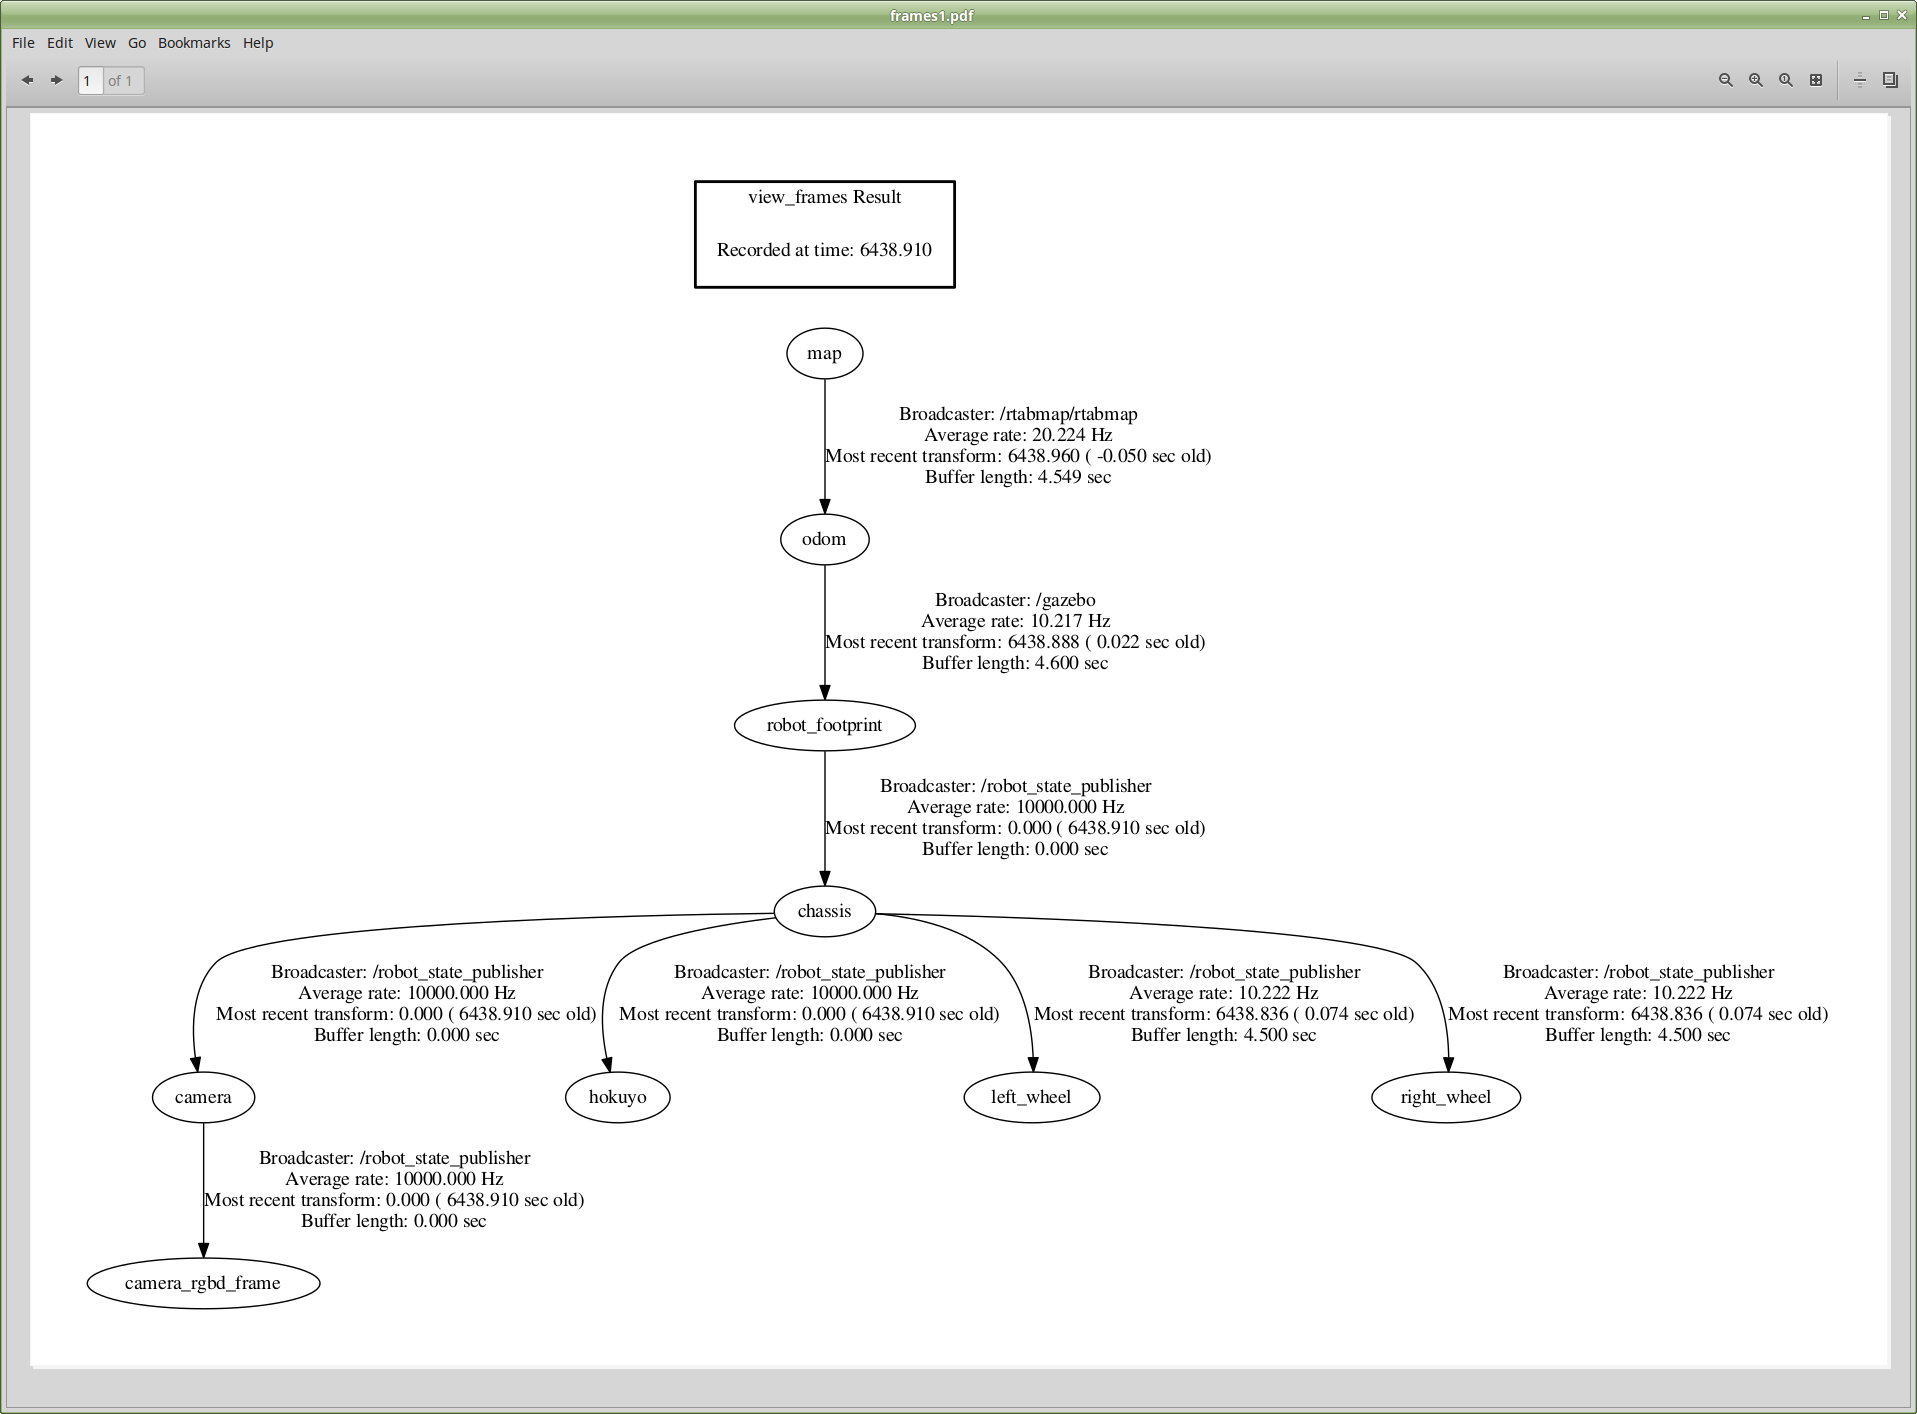
\includegraphics[width=\linewidth]{Assets/Frames1_ScreenShot_2019-02-12_16-25-23.png}
      \caption{CielBot Transform Tree}
      \label{fig:tftree}
\end{figure}


\subsection{Custom World Config}

\section{Results}
Results


\section{Discussion}
Discussion

\section{Conclusion / Future work}
Conclusion


\end{document}